\chapter{Исследовательский раздел}

\section{Технические характеристики}

Технические характеристики устройства, на котором запускалась программа:

\begin{enumerate}
	\item операционная система Ubuntu, 22.04.4~\cite{ubuntu} c версией ядра 5.19.17;
	\item память 16 Гайт;
	\item процессор 2,5 ГГц 4‑дерный процессор Intel Core i5-10300H~\cite{intel}.
\end{enumerate}

\section{Исследование работы программы}

Для исследования работы были разработаны вспомогательные программы.

\begin{enumerate}
	\item программа, которая создает процесс-потомок и посылает ему сигнал;
	\item программа, в которой предок и потомок обмениваются сообщениями через программный канал;
	\item программа на основе задачи <<производство--потребление>>;
	\item программа на основе задачи <<читатели--писатели>>.
\end{enumerate}

Весь код вспомогательных программ представлен в Приложении А.

На рисунке~\ref{img:example-general} продемонстрирована работа загружамого модуля при чтении из файла general.

\begin{figure}[h]
	\centering
	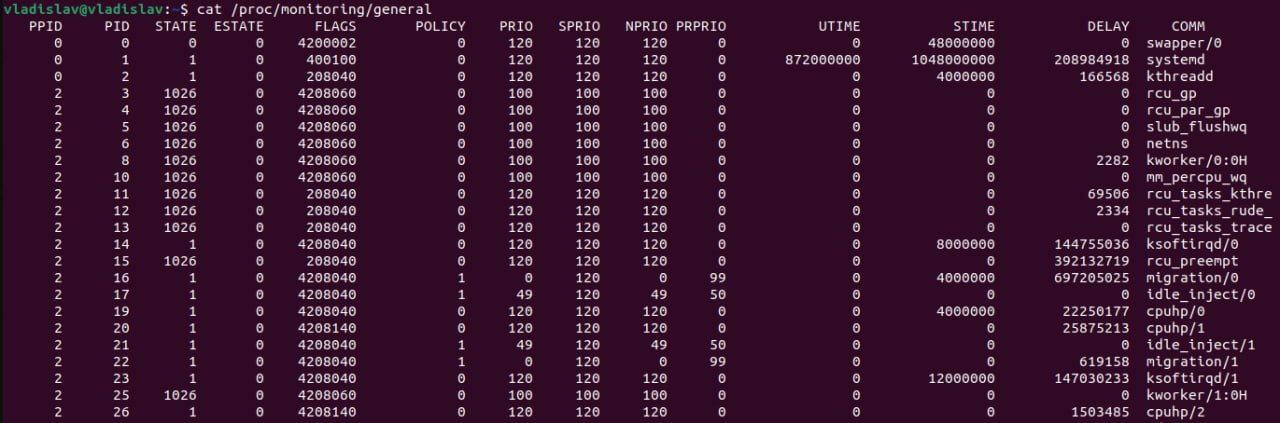
\includegraphics[width=0.9\textwidth]{img/example-general}
	\caption{Демонстрация работы программы при чтении из файла \texttt{general}}
	\label{img:example-general}
\end{figure}

На рисунке~\ref{img:example-memory} продемонстрирована работа загружамого модуля при чтении из файла memory.

\begin{figure}[h]
	\centering
	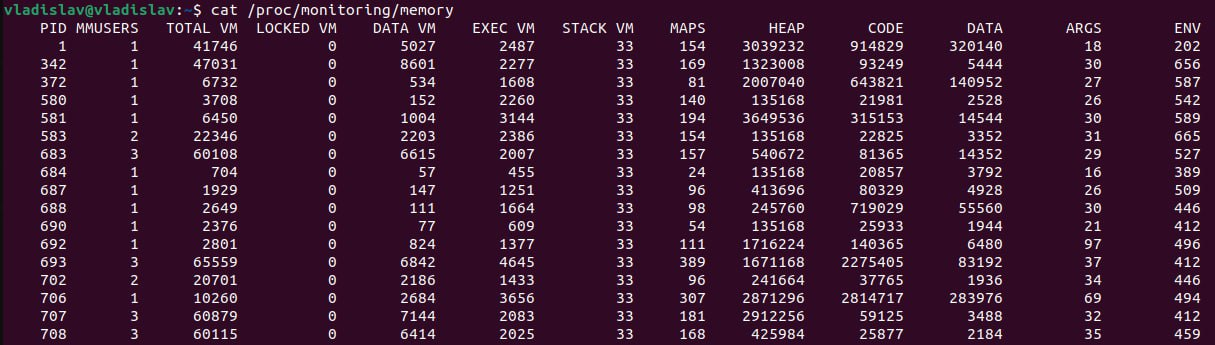
\includegraphics[width=0.9\textwidth]{img/example-memory}
	\caption{Демонстрация работы программы при чтении из файла \texttt{memory}}
	\label{img:example-memory}
\end{figure}

На рисунке~\ref{img:example-maps} продемонстрирована работа загружамого модуля при записи в файл идентификатора процесса и чтении из файла maps.

\begin{figure}[h]
	\centering
	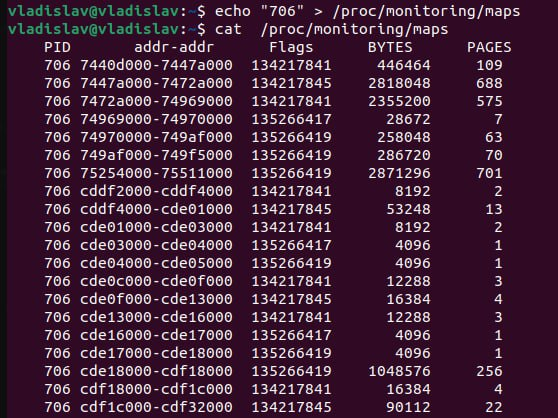
\includegraphics[width=0.7\textwidth]{img/example-maps}
	\caption{Демонстрация работы программы при записи в файл и чтении из файла \texttt{maps}}
	\label{img:example-maps}
\end{figure}

\clearpage

На рисунке~\ref{img:example-sighand} продемонстрирована работа загружамого модуля при чтении из файла sighands.

\begin{figure}[h]
	\centering
	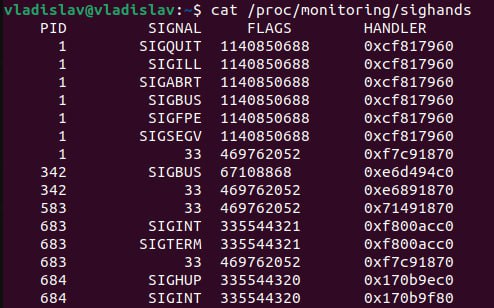
\includegraphics[width=0.7\textwidth]{img/example-sighand}
	\caption{Демонстрация работы программы при записи в файл и чтении из файла \texttt{sighands}}
	\label{img:example-sighand}
\end{figure}

На рисунке~\ref{img:program-signal} представлен запуск вспомогательной програмы 1, в результате которой был отправлен сигнал. 
На рисунке~\ref{img:example-signal} представлено чтение из файла \texttt{signals}.

\begin{figure}[h]
	\centering
	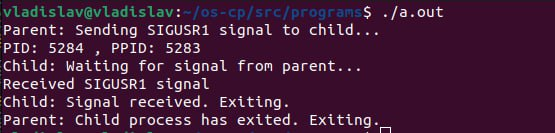
\includegraphics[width=0.7\textwidth]{img/program-signal}
	\caption{Демонстрация работы вспомогательной работы 1}
	\label{img:program-signal}
\end{figure}

\begin{figure}[h]
	\centering
	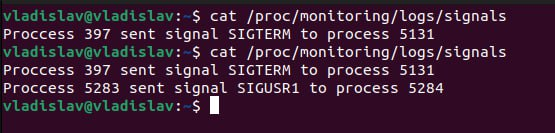
\includegraphics[width=0.7\textwidth]{img/example-signal}
	\caption{Демонстрация работы программы чтении из файла \texttt{signals}}
	\label{img:example-signal}
\end{figure}

\clearpage

На рисунке~\ref{img:program-pipe} представлен запуск вспомогательной програмы 2, в результате два процесса обмениваются сообщениями через программный канал. 
На рисунке~\ref{img:example-pipe} представлено чтение из файла \texttt{pipe}.

\begin{figure}[h]
	\centering
	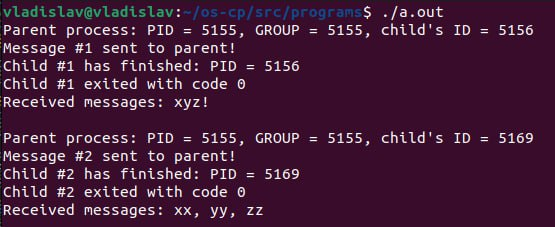
\includegraphics[width=0.7\textwidth]{img/program-pipe}
	\caption{Демонстрация работы вспомогательной работы 2}
	\label{img:program-pipe}
\end{figure}

\begin{figure}[h]
	\centering
	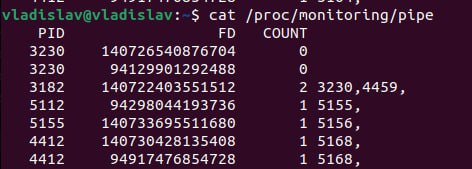
\includegraphics[width=0.7\textwidth]{img/example-pipe}
	\caption{Демонстрация работы программы чтении из файла \texttt{pipe}}
	\label{img:example-pipe}
\end{figure}

На рисунке~\ref{img:program-pc}--\ref{img:program-wr} представлен запуск вспомогательной програмы 2 и 3, а на рисунке~\ref{img:example-sem-shm} представлено чтение из файлов \texttt{sem} и \texttt{shm}.

\begin{figure}[h]
	\centering
	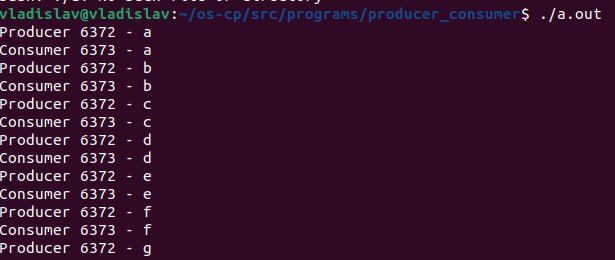
\includegraphics[width=0.7\textwidth]{img/program-p-c}
	\caption{Демонстрация работы вспомогательной работы 2}
	\label{img:program-pc}
\end{figure}

\clearpage

\begin{figure}[h]
	\centering
	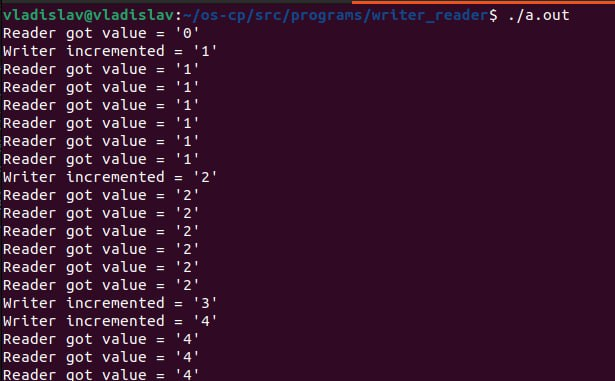
\includegraphics[width=0.55\textwidth]{img/program-r-w}
	\caption{Демонстрация работы вспомогательной работы 3}
	\label{img:program-wr}
\end{figure}

\begin{figure}[h]
	\centering
	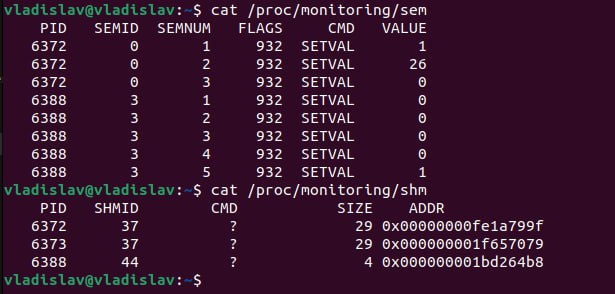
\includegraphics[width=0.55\textwidth]{img/example-sem-shm}
	\caption{Демонстрация работы программы чтении из файлов \texttt{sem} и \texttt{shm}}
	\label{img:example-sem-shm}
\end{figure}

\begin{figure}[h]
	\centering
	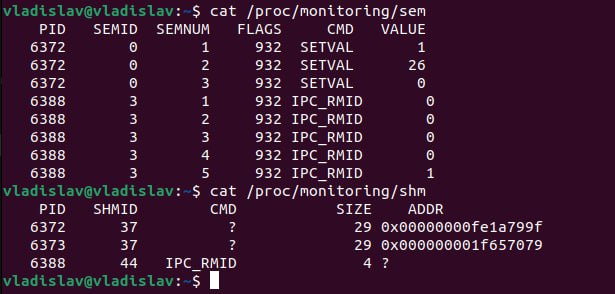
\includegraphics[width=0.55\textwidth]{img/example-sem-shm-2}
	\caption{Демонстрация работы программы чтении из файлов \texttt{sem} и \texttt{shm}}
	\label{img:example-sem-shm-2}
\end{figure}